%!TEX root = ./main.tex
%!TEX program = xelatex
% =====================================================================
%  06 - PHỤ LỤC
% =====================================================================
\chapter{Mã nguồn firmware}
\label{app:firmware}

Mã nguồn đầy đủ được lưu tại kho GitHub của nhóm:\\
\url{https://github.com/1m4n00b6292/ME4169-Microprocessor-Final-term-Project}. Tên tệp và chú thích trong mã nguồn vẫn giữ tên dự án cũ ``VI XU LY''.

\section{Cấu hình}
\lstinputlisting[caption={config.h},label={lst:config}]{firmware/src/config.h}
\lstinputlisting[language={},caption={platformio.ini}]{firmware/platformio.ini}

\section{Lớp điểm vào và ứng dụng}
\lstinputlisting[language=C++,caption={main.cpp}]{firmware/src/main.cpp}
\lstinputlisting[language=C++,caption={app.h}]{firmware/src/app.h}
\lstinputlisting[language=C++,caption={app.cpp}]{firmware/src/app.cpp}

\section{Lớp điều khiển}
\lstinputlisting[caption={motion.h}]{firmware/src/motion.h}
\lstinputlisting[caption={motion.c}]{firmware/src/motion.c}

\section{Lớp driver}
\lstinputlisting[caption={motor.h}]{firmware/src/motor.h}
\lstinputlisting[caption={motor.c}]{firmware/src/motor.c}
\lstinputlisting[language=C++,caption={encoder\_mini.h}]{firmware/src/encoder_mini.h}
\lstinputlisting[language=C++,caption={encoder\_mini.cpp}]{firmware/src/encoder_mini.cpp}
\lstinputlisting[caption={button.h}]{firmware/src/button.h}
\lstinputlisting[caption={button.c}]{firmware/src/button.c}
\lstinputlisting[caption={uart.h}]{firmware/src/uart.h}
\lstinputlisting[caption={uart.c}]{firmware/src/uart.c}
\lstinputlisting[caption={adc.h}]{firmware/src/adc.h}
\lstinputlisting[caption={adc.c}]{firmware/src/adc.c}
\lstinputlisting[caption={st7735\_mini.h}]{firmware/src/st7735_mini.h}
\lstinputlisting[caption={st7735\_mini.c}]{firmware/src/st7735_mini.c}

\chapter{Sơ đồ nguyên lý}
\label{app:schematic}
Sơ đồ nguyên lý đầy đủ của \proj{} (xuất từ KiCad) được trình bày ở trang sau, xoay ngang khổ A4.

\begin{center}
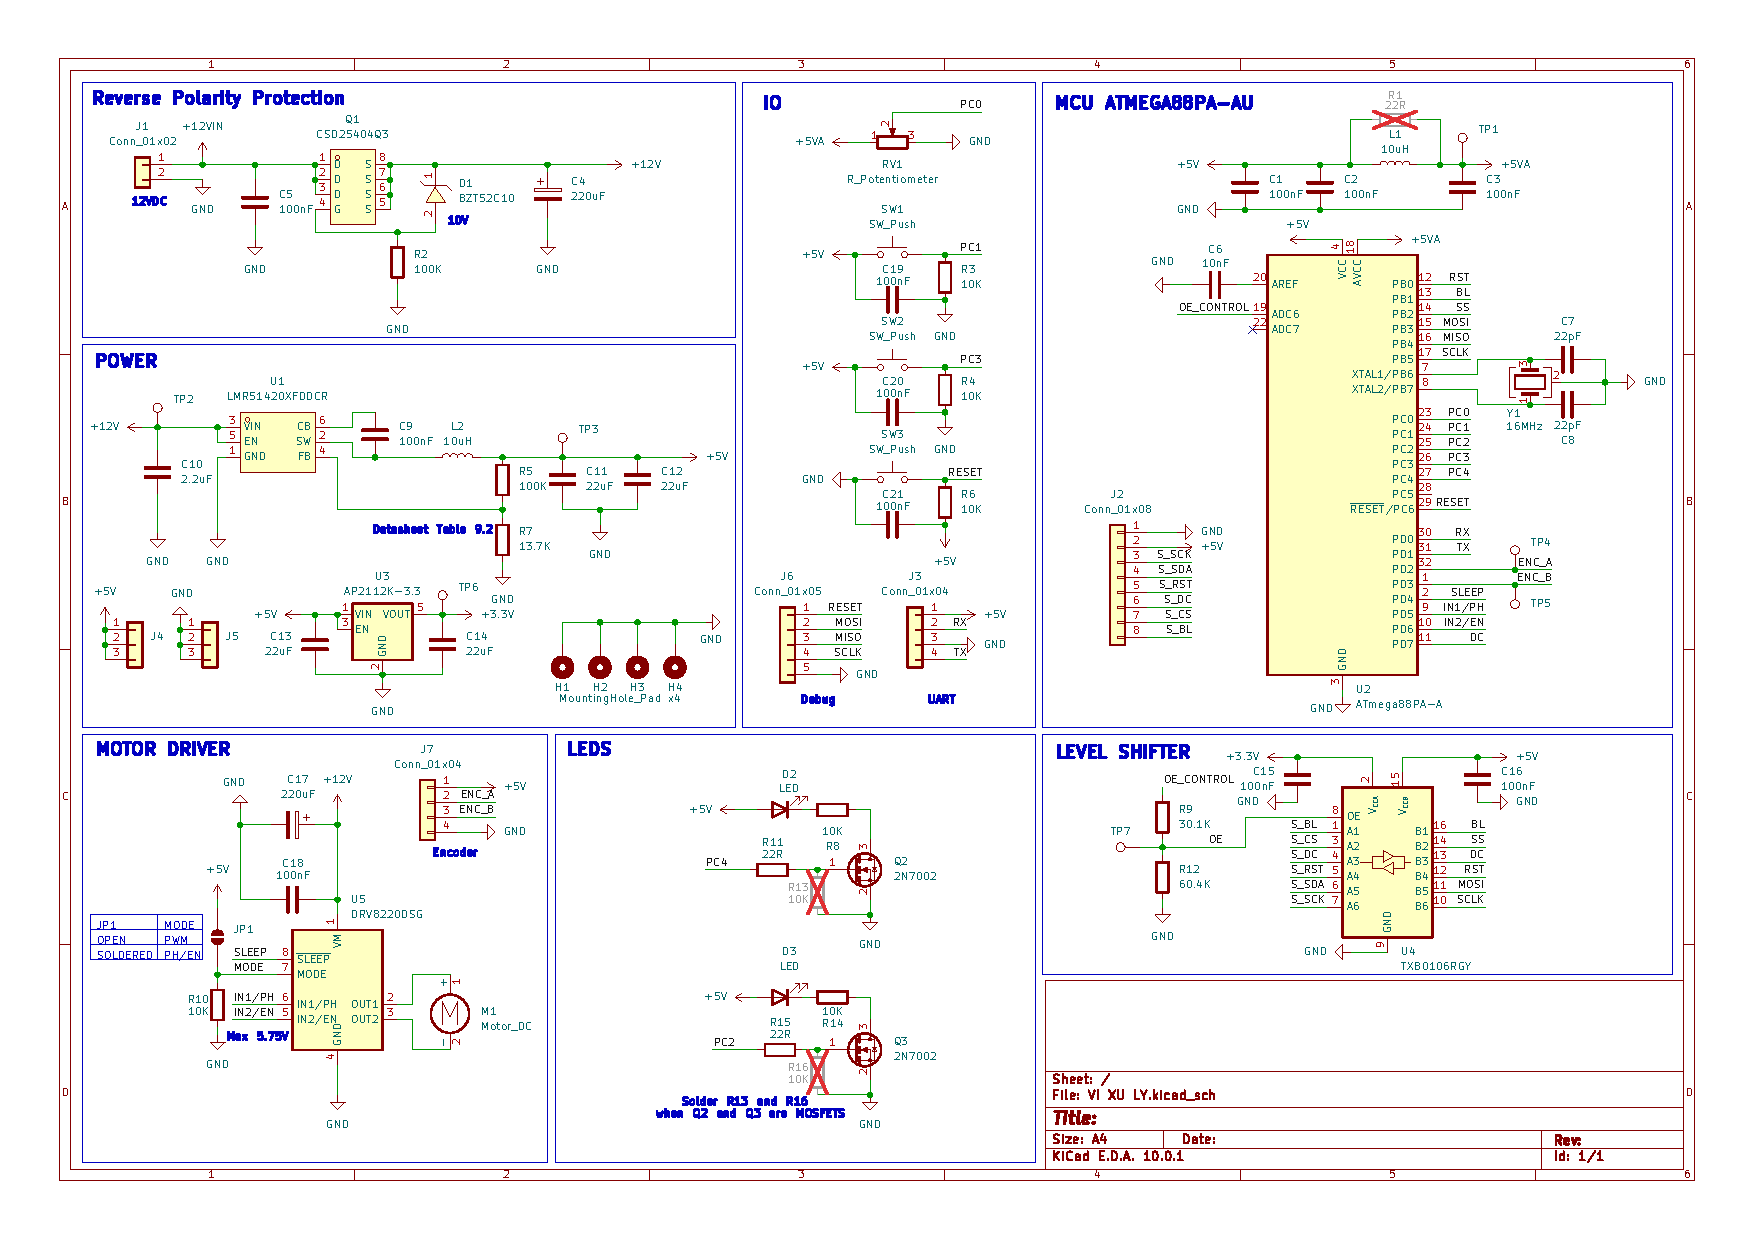
\includegraphics[height=\linewidth,angle=90,page=1]{sch/VIXULY_schematic.pdf}
\end{center}

\chapter{Danh sách linh kiện đầy đủ (BOM)}
\label{app:bom}

Bảng~\ref{tab:bom} là danh sách linh kiện đầy đủ của \proj{}, bao gồm cả linh kiện thụ động, nút nhấn và đầu nối, được trích trực tiếp từ sơ đồ nguyên lý KiCad và nhóm theo khối chức năng.

{\small
\begin{longtable}{@{}>{\raggedright\arraybackslash}p{2.2cm}>{\raggedright\arraybackslash}p{3.5cm}>{\raggedright\arraybackslash}p{2.8cm}c>{\raggedright\arraybackslash}p{5.1cm}@{}}
\caption{Danh sách linh kiện đầy đủ (BOM) của \proj}\label{tab:bom}\\
\toprule
\textbf{Ký hiệu} & \textbf{Giá trị / Mã} & \textbf{Vỏ (footprint)} & \textbf{SL} & \textbf{Chức năng}\\
\midrule\endfirsthead
\toprule
\textbf{Ký hiệu} & \textbf{Giá trị / Mã} & \textbf{Vỏ (footprint)} & \textbf{SL} & \textbf{Chức năng}\\
\midrule\endhead
\bottomrule\endfoot
\multicolumn{5}{@{}l}{\cellcolor{blkfill}\textit{Khối xử lý trung tâm}}\\
U2 & ATmega88PA-A & TQFP-32 & 1 & Vi điều khiển chính\\
Y1 & \SI{16}{\mega\hertz} & SMD 3225 & 1 & Thạch anh dao động\\
C7, C8 & \SI{22}{\pico\farad} & 0603 & 2 & Tụ tải thạch anh\\
L1 / R1 & \SI{10}{\micro\henry} / \SI{22}{\ohm} & 0603 & 2 & Lọc nguồn AVCC (+5VA)\\
C1--C3, C6 & \SI{100}{\nano\farad}, \SI{10}{\nano\farad} & 0603 & 4 & Tụ thoát VCC/AVCC/AREF\\
SW3, R6, C21 & Nút nhấn, \SI{10}{\kilo\ohm}, \SI{100}{\nano\farad} & B3F, 0603 & 3 & Mạch RESET\\
\multicolumn{5}{@{}l}{\cellcolor{pwrfill}\textit{Khối nguồn và bảo vệ}}\\
Q1 & CSD25404Q3 & VSON-8 3,3$\times$3,3 & 1 & P-MOSFET chống ngược cực\\
D1 & BZT52C10 & SOD-123 & 1 & Zener kẹp $V_{GS}$ của Q1\\
R2 & \SI{100}{\kilo\ohm} & 0603 & 1 & Điện trở cực cổng Q1\\
U1 & LMR51420XFDDCR & SOT-23-6 & 1 & Buck đồng bộ \SI{12}{\volt}$\to$\SI{5}{\volt}\\
L2 & \SI{10}{\micro\henry} & IHLP-1616 & 1 & Cuộn cảm buck\\
R5, R7 & \SI{100}{\kilo\ohm}, \SI{13.7}{\kilo\ohm} & 0603 & 2 & Cầu phân áp hồi tiếp (FB)\\
C9, C10, C11, C12 & \SI{100}{\nano\farad}, \SI{2.2}{\micro\farad}, 2$\times$\SI{22}{\micro\farad} & 0603/1206 & 4 & Bootstrap, tụ vào, tụ ra\\
U3 & AP2112K-3.3 & SOT-23-5 & 1 & LDO \SI{3.3}{\volt} / \SI{600}{\milli\ampere}\\
C13, C14 & \SI{22}{\micro\farad} & 1206 & 2 & Tụ vào/ra LDO\\
C4, C17 & \SI{220}{\micro\farad} & Hóa 6,3$\times$7,7 & 2 & Tụ bulk bus \SI{12}{\volt}\\
\multicolumn{5}{@{}l}{\cellcolor{blkfill}\textit{Khối công suất}}\\
U5 & DRV8220DSG & WSON-8 2$\times$2 & 1 & Cầu H \SI{18}{\volt}/\SI{1.76}{\ampere}\\
JP1, R10 & Jumper hàn, \SI{10}{\kilo\ohm} & -- & 2 & Chọn chế độ PWM / PH-EN\\
C18 & \SI{100}{\nano\farad} & 0603 & 1 & Tụ thoát VM\\
M1 & Domino 2 chân & MKDS 5,08 & 1 & Đầu ra động cơ\\
\multicolumn{5}{@{}l}{\cellcolor{iofill}\textit{Khối giao diện}}\\
U4 & TXB0106RGY & VQFN-16 & 1 & Chuyển mức \SI{5}{\volt}$\leftrightarrow$\SI{3.3}{\volt} cho TFT\\
R9, R12 & \SI{30.1}{\kilo\ohm}, \SI{60.4}{\kilo\ohm} & 0603 & 2 & Phân áp chân OE\\
C15, C16 & \SI{100}{\nano\farad} & 0603 & 2 & Tụ thoát VCCA/VCCB\\
RV1 & Chiết áp Alps RK097 & -- & 1 & Đặt tốc độ\\
SW1, SW2 & Nút nhấn Omron B3F & -- & 2 & Nút RUN, STOP\\
R3, R4, C19, C20 & \SI{10}{\kilo\ohm}, \SI{100}{\nano\farad} & 0603 & 4 & Kéo xuống + lọc RC nút nhấn\\
D2, D3 & LED & 1206 & 2 & LED STOP, RUN\\
Q2, Q3 & 2N7002 & SOT-23 & 2 & Khóa LED\\
R8, R11, R13--R16 & \SI{10}{\kilo\ohm}, \SI{22}{\ohm} & 0603 & 6 & Trở hạn dòng LED, trở cổng\\
\multicolumn{5}{@{}l}{\cellcolor{swfill}\textit{Đầu nối và cơ khí}}\\
J1 & Domino 2 chân & MKDS 5,08 & 1 & Đầu vào nguồn \SI{12}{\volt}\\
J2 & Header cái 1$\times$8 & 2,54 mm & 1 & Module TFT WeAct ST7735\\
J3 & JST-XH 4 chân & 2,50 mm & 1 & UART\\
J6 & JST-XH 5 chân & 2,50 mm & 1 & Nạp ISP\\
J7 & JST-XH 4 chân & 2,50 mm & 1 & Encoder\\
J4, J5 & Header 1$\times$3 & 2,54 mm & 2 & Đầu chờ +5V / GND\\
TP1--TP7 & Test point & $\varnothing$\SI{1}{\milli\metre} & 7 & Điểm đo\\
H1--H4 & Lỗ M3 & $\varnothing$\SI{3.2}{\milli\metre} & 4 & Lỗ bắt vít\\
\end{longtable}
}

\chapter{Layout mạch in}
\label{app:layout}

\begin{figure}[H]
\centering
\hinh[0.95\linewidth]{figures/Layout_Front.png}{Layout lớp trên}
\caption{Layout lớp trên (F.Cu) -- kích thước đầy đủ}
\end{figure}

\begin{figure}[H]
\centering
\hinh[0.95\linewidth]{figures/Layout_Back.png}{Layout lớp dưới}
\caption{Layout lớp dưới (B.Cu) -- kích thước đầy đủ}
\end{figure}

\begin{table}[H]
\centering\small
\caption{Danh sách tệp sản xuất (Gerber)}
\begin{tabular}{@{}ll@{}}
\toprule
\textbf{Tệp} & \textbf{Nội dung}\\
\midrule
\texttt{VI XU LY-F\_Cu.gbr} / \texttt{-B\_Cu.gbr} & Lớp đồng trên / dưới\\
\texttt{VI XU LY-F\_Mask.gbr} / \texttt{-B\_Mask.gbr} & Mặt nạ hàn\\
\texttt{VI XU LY-F\_Silkscreen.gbr} / \texttt{-B\_Silkscreen.gbr} & Lớp in lụa\\
\texttt{VI XU LY-F\_Paste.gbr} / \texttt{-B\_Paste.gbr} & Lớp kem hàn (stencil)\\
\texttt{VI XU LY-Edge\_Cuts.gbr} & Đường viền bo mạch\\
\texttt{VI XU LY.drl}, \texttt{VI XU LY-drl\_map.gbr} & Tệp khoan và bản đồ khoan\\
\texttt{VI XU LY-job.gbrjob} & Tệp mô tả công việc (Gerber job)\\
\bottomrule
\end{tabular}
\end{table}

\chapter{Tài liệu tham khảo}
\label{app:docs}

\begingroup
\makeatletter\let\chapter\@gobbletwo\makeatother
\begin{thebibliography}{99}
\bibitem{atmega} Microchip Technology, \emph{ATmega48PA/88PA/168PA/328P -- 8-bit AVR Microcontroller with 4/8/16/32K Bytes In-System Programmable Flash}, Datasheet.
\bibitem{drv8220} Texas Instruments, \emph{DRV8220 18-V H-Bridge Motor Driver with PWM, PH/EN, and Half-Bridge Control Interfaces and Low-Power Sleep Mode}, SLVSFU5B, 2021.
\bibitem{lmr51420} Texas Instruments, \emph{LMR51420 SIMPLE SWITCHER\textsuperscript{\textregistered} 4.5-V to 36-V, 2-A Synchronous Buck Converter in a SOT-23 Package}, SLUSEF6C, 2022.
\bibitem{csd25404} Texas Instruments, \emph{CSD25404Q3 --20 V P-Channel NexFET\texttrademark{} Power MOSFET}, SLPS570, 2015.
\bibitem{txb0106} Texas Instruments, \emph{TXB0106 6-Bit Bidirectional Level-Shifting and Voltage Translator With Auto-Direction Sensing}, SCES709C, 2025.
\bibitem{ap2112} Diodes Incorporated, \emph{AP2112 600mA CMOS LDO Regulator with Enable}, Datasheet.
\bibitem{st7735} Sitronix, \emph{ST7735S 132RGB$\times$162dot 262K Color with Frame Memory Single-Chip TFT Controller/Driver}, Datasheet.
\bibitem{weact} WeAct Studio, \emph{WeAct ST7735 TFT Module}, \url{https://github.com/WeActStudio/WeAct-ST7735}.
\bibitem{pio} PlatformIO, \emph{PlatformIO Documentation -- Atmel AVR platform}, \url{https://docs.platformio.org}.
\bibitem{arduinoisp} Arduino, \emph{Arduino as ISP and Arduino Bootloaders}, \url{https://docs.arduino.cc/built-in-examples/arduino-isp/ArduinoISP}.
\bibitem{kicad} KiCad EDA, \emph{KiCad Documentation}, \url{https://docs.kicad.org}.
\bibitem{ogata} K. Ogata, \emph{Modern Control Engineering}, 5th ed., Prentice Hall, 2010.
\bibitem{astrom} K. J. Åström, T. Hägglund, \emph{Advanced PID Control}, ISA, 2006.
\bibitem{repo} Nhóm thực hiện, \emph{ME4169 Microprocessor Final term project -- mã nguồn và thiết kế}, \url{https://github.com/1m4n00b6292/ME4169-Microprocessor-Final-term-Project}.
\end{thebibliography}
\endgroup
